\documentclass{scrartcl}
\usepackage[mathletters]{ucs}
\usepackage[utf8x]{inputenc}
\usepackage{amssymb}
\usepackage{amsmath}
\usepackage[usenames]{color}
\usepackage{hyperref}
\usepackage{wasysym}
\usepackage{graphicx}
\usepackage[normalem]{ulem}
\usepackage{enumerate}

\usepackage{listings}

\lstset{ %
basicstyle=\footnotesize,       % the size of the fonts that are used for the code
showspaces=false,               % show spaces adding particular underscores
showstringspaces=false,         % underline spaces within strings
showtabs=false,                 % show tabs within strings adding particular underscores
frame=single,                   % adds a frame around the code
tabsize=2,                      % sets default tabsize to 2 spaces
breaklines=true,                % sets automatic line breaking
breakatwhitespace=false,        % sets if automatic breaks should only happen at whitespace
}


\title{camera position validation}
\date{dinsdag 08 december 2020}
\author{}

\begin{document}

\maketitle

		\section{camera position validation}

Created woensdag 18 november 2020



\subsection{Information}

The next data input structure is made:

	\begin{itemize}
	\item 20 train images
	\item 10 validation images
	\item 10 test images
	\end{itemize}


These images will go through different algorithms multiple times and the outputs are verified for every different algorithm.



\subsection{papers}



\begin{enumerate}[1]
\item A Comprehensive Study on Deep Image Classification with Small Datasets
	\begin{enumerate}[a]
	\item short comparison of the amount of convolutional layers to be used in the network (5 is optimal)
	\item comparison on datasets: Caltech101, CIFAR10
	\item also transfer learning also around 5 convolutional layers is the optimum
	\item network architecture
		\begin{enumerate}[1]
		\item from scratch:
		\end{enumerate}
	\end{enumerate}
\end{enumerate}
			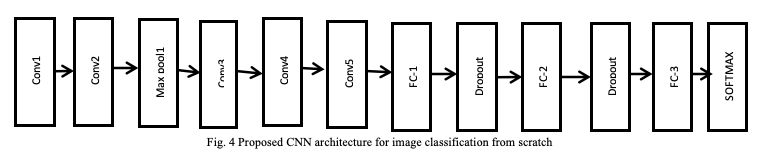
\includegraphics[]{./camera_position_validation/paper1_arch_fromscratch.png}
			
		\begin{enumerate}[1]
		\setcounter{enumi}{1}
		\item transfer learning pretrained on VGG16 with imagenet dataset
		\end{enumerate}
			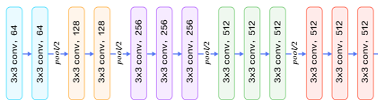
\includegraphics[]{./camera_position_validation/paper1_arch_transferlearning.png}
			
\begin{enumerate}[1]
\setcounter{enumi}{1}
\item Deep learning for image classifification on very small datasets using transfer learning
	\begin{enumerate}[a]
	\item creation of an image classification network with context of where it comes from
		\begin{enumerate}[1]
		\item alexnet vs googlenet vs vgg and the history
		\item displays keras code to create the same models
		\item architecture for models is shown
		\item niet super interessant gezien hier nog steeds wordt gewerkt op 6000 fotos van katten en honden, wel een indicatie dat deep learning gaat met weinig data
		\end{enumerate}
	\end{enumerate}
\end{enumerate}




\begin{enumerate}[1]
\setcounter{enumi}{2}
\item \href{https://paperswithcode.com/task/small-data}{https://paperswithcode.com/task/small-data}
	\begin{enumerate}[a]
	\item interesting papers with small datasets
	\end{enumerate}
\end{enumerate}


\begin{enumerate}[1]
\setcounter{enumi}{3}
\item A survey of the recent architectures of deep convolutional neural networks
	\begin{enumerate}[a]
	\item overview of almost all neural networks with their strengths and weaknesses
	\end{enumerate}
\end{enumerate}


\begin{enumerate}[1]
\setcounter{enumi}{4}
\item SDD-CNN: Small data-driven convolution neural networks for subtle roller defect inspection
	\begin{enumerate}[a]
	\item very interesting paper detects faults in bearing rollers. 
	\item Using very little data
	\item results with from scratch training best with SDD-inception v3 and SDD-resnet18
	\item SDD-VGG16 gets good results, but with long trainin time
	\end{enumerate}
\end{enumerate}


In most seen papers a very low learning rate 

0.0005 









\end{document}
